% !TEX program = xelatex
% 编译: 在 docs/实验报告/ 目录下  xelatex 实验报告.tex
% 模板沿用 College_Physics_Labs/非平衡电桥 的浙大实验报告模板; 图片相对路径见 \graphicspath
\documentclass[12pt,a4paper]{ctexart}
\usepackage[margin=2cm]{geometry}
\usepackage{graphicx}
\usepackage{amsmath}
\usepackage{amssymb}
\usepackage{physics}
\usepackage{booktabs}
\usepackage{array}
\usepackage{wrapfig}
\usepackage{enumitem}
\usepackage{caption}
\captionsetup{font=footnotesize}            % 图/表 caption 改小到放大前字号(10pt)
\usepackage{xcolor}
\usepackage{listings}
\lstset{
  basicstyle=\ttfamily\footnotesize,
  keywordstyle=\color{blue!70!black},
  commentstyle=\color{green!40!black}\itshape,
  stringstyle=\color{red!60!black},
  numbers=left, numberstyle=\tiny\color{gray}, numbersep=7pt,
  breaklines=true, frame=single, framesep=4pt, xleftmargin=1.6em,
  showstringspaces=false, tabsize=4, columns=fullflexible, basewidth=0.5em,
  extendedchars=true,
}
\renewcommand{\lstlistingname}{代码}
\usepackage{fancyhdr}
\newcommand{\myspace}[1]{\par\vspace{#1\baselineskip}}
\newcommand{\code}[1]{\texttt{#1}}

\graphicspath{{figures/}{../../assets/}{../../design-tool/docs/images/}}

\pagestyle{fancy}
\fancyhf{}
\fancyfoot[C]{\thepage}
\renewcommand{\headrulewidth}{0pt}
\renewcommand{\footrulewidth}{0pt}

\usepackage{hyperref}
\hypersetup{colorlinks=true,linkcolor=blue,filecolor=magenta,urlcolor=cyan,
            pdftitle={SpiRobs 绳驱动连续体机械臂实验报告}}

\usepackage{titlesec}
% 自定义字号指令
\newcommand{\chuhao}{\fontsize{42pt}{48pt}\selectfont}
\newcommand{\xiaochu}{\fontsize{36pt}{42pt}\selectfont}
\newcommand{\xiaoer}{\fontsize{18pt}{21.6pt}\selectfont}
\newcommand{\sanhao}{\fontsize{16pt}{20pt}\selectfont}
\newcommand{\xiaosan}{\fontsize{15pt}{18pt}\selectfont}
\newcommand{\sihao}{\fontsize{14pt}{18pt}\selectfont}
\newcommand{\xiaosi}{\fontsize{12pt}{16pt}\selectfont}
\newcommand{\wuhao}{\fontsize{10.5pt}{12.6pt}\selectfont}

% section 用中文数字编号: 一、二、...
\titleformat{\section}
  {\normalfont\Large\bfseries}
  {\zhnum{section}、}{0pt}{}

\begin{document}

\vspace*{36pt}

% ===================== 封面 =====================
\begin{center}
    
\includegraphics[width=9cm]{head.png}

    \xiaochu\textbf{实验报告}
    \vspace{13pt}\vspace{13pt}\vspace{13pt}\vspace{13pt}

    \sanhao\textbf{实验名称：\underline{\makebox[8cm]{ SpiRobs 绳驱动连续体机械臂 }}} \\[10pt]
    \sanhao\textbf{课程名称：\underline{\makebox[8cm]{ 软体仿生机器人与智能材料 }}} \\[10pt]
    \sanhao\textbf{指导教师：\underline{\makebox[8cm]{ 李铁风/郑兴文/周方浩/陆豪健 }}} \\[20pt]

    \myspace{6}

    \sihao\textbf{班级：\underline{\makebox[6cm]{机器人工程2402}}} \\[10pt]
    \sihao\textbf{姓名：\underline{\makebox[6cm]{毛挺}}} \\[10pt]
    \sihao\textbf{学号：\underline{\makebox[6cm]{3240104043}}} \\[30pt]

    \sihao\textbf{实验日期：\underline{\makebox[1.2cm]{2026}}年\underline{\makebox[0.8cm]{6}}月\underline{\makebox[0.8cm]{14}}日}

    \vspace{18pt}
    \sihao\textbf{浙江大学 \ 《软体仿生机器人与智能材料》课程}
\end{center}

\newpage

% ===================== 摘要 =====================
\noindent\hspace*{2em}\textbf{摘要}：本实验围绕 SpiRobs 绳驱动连续体机械臂，完成了从\textbf{对数螺旋仿生结构设计}、\textbf{TPU 柔性骨架 3D 打印与装配}、
\textbf{三绳驱动模块搭建}到\textbf{联动控制软件实现与运动标定}的完整链路。结构上采用对数螺旋
$r=a\,e^{b\theta}$ 离散展开的柔性主体，三根驱动绳按 $120^\circ$ 分布；驱动上使用三台 MKS SERVO35D 闭环步进电机经
RS485 总线由上位机统一控制。控制上将整条触手抽象为\textbf{三自由度任务空间}（弯曲方向、弯曲大小、整体收缩），
建立恒曲率腱驱动映射，并针对真机"放线过度致绳松"的问题设计了\textbf{非线性收放线整形}（收线线性、放线随弯曲量超线性）。
样机实现了全向弯曲与从上/下方对物体的柔性包络抓取。本文给出设计参数、控制原理、标定方法、实验结果与误差分析。

\begin{figure}[htbp]
\centering
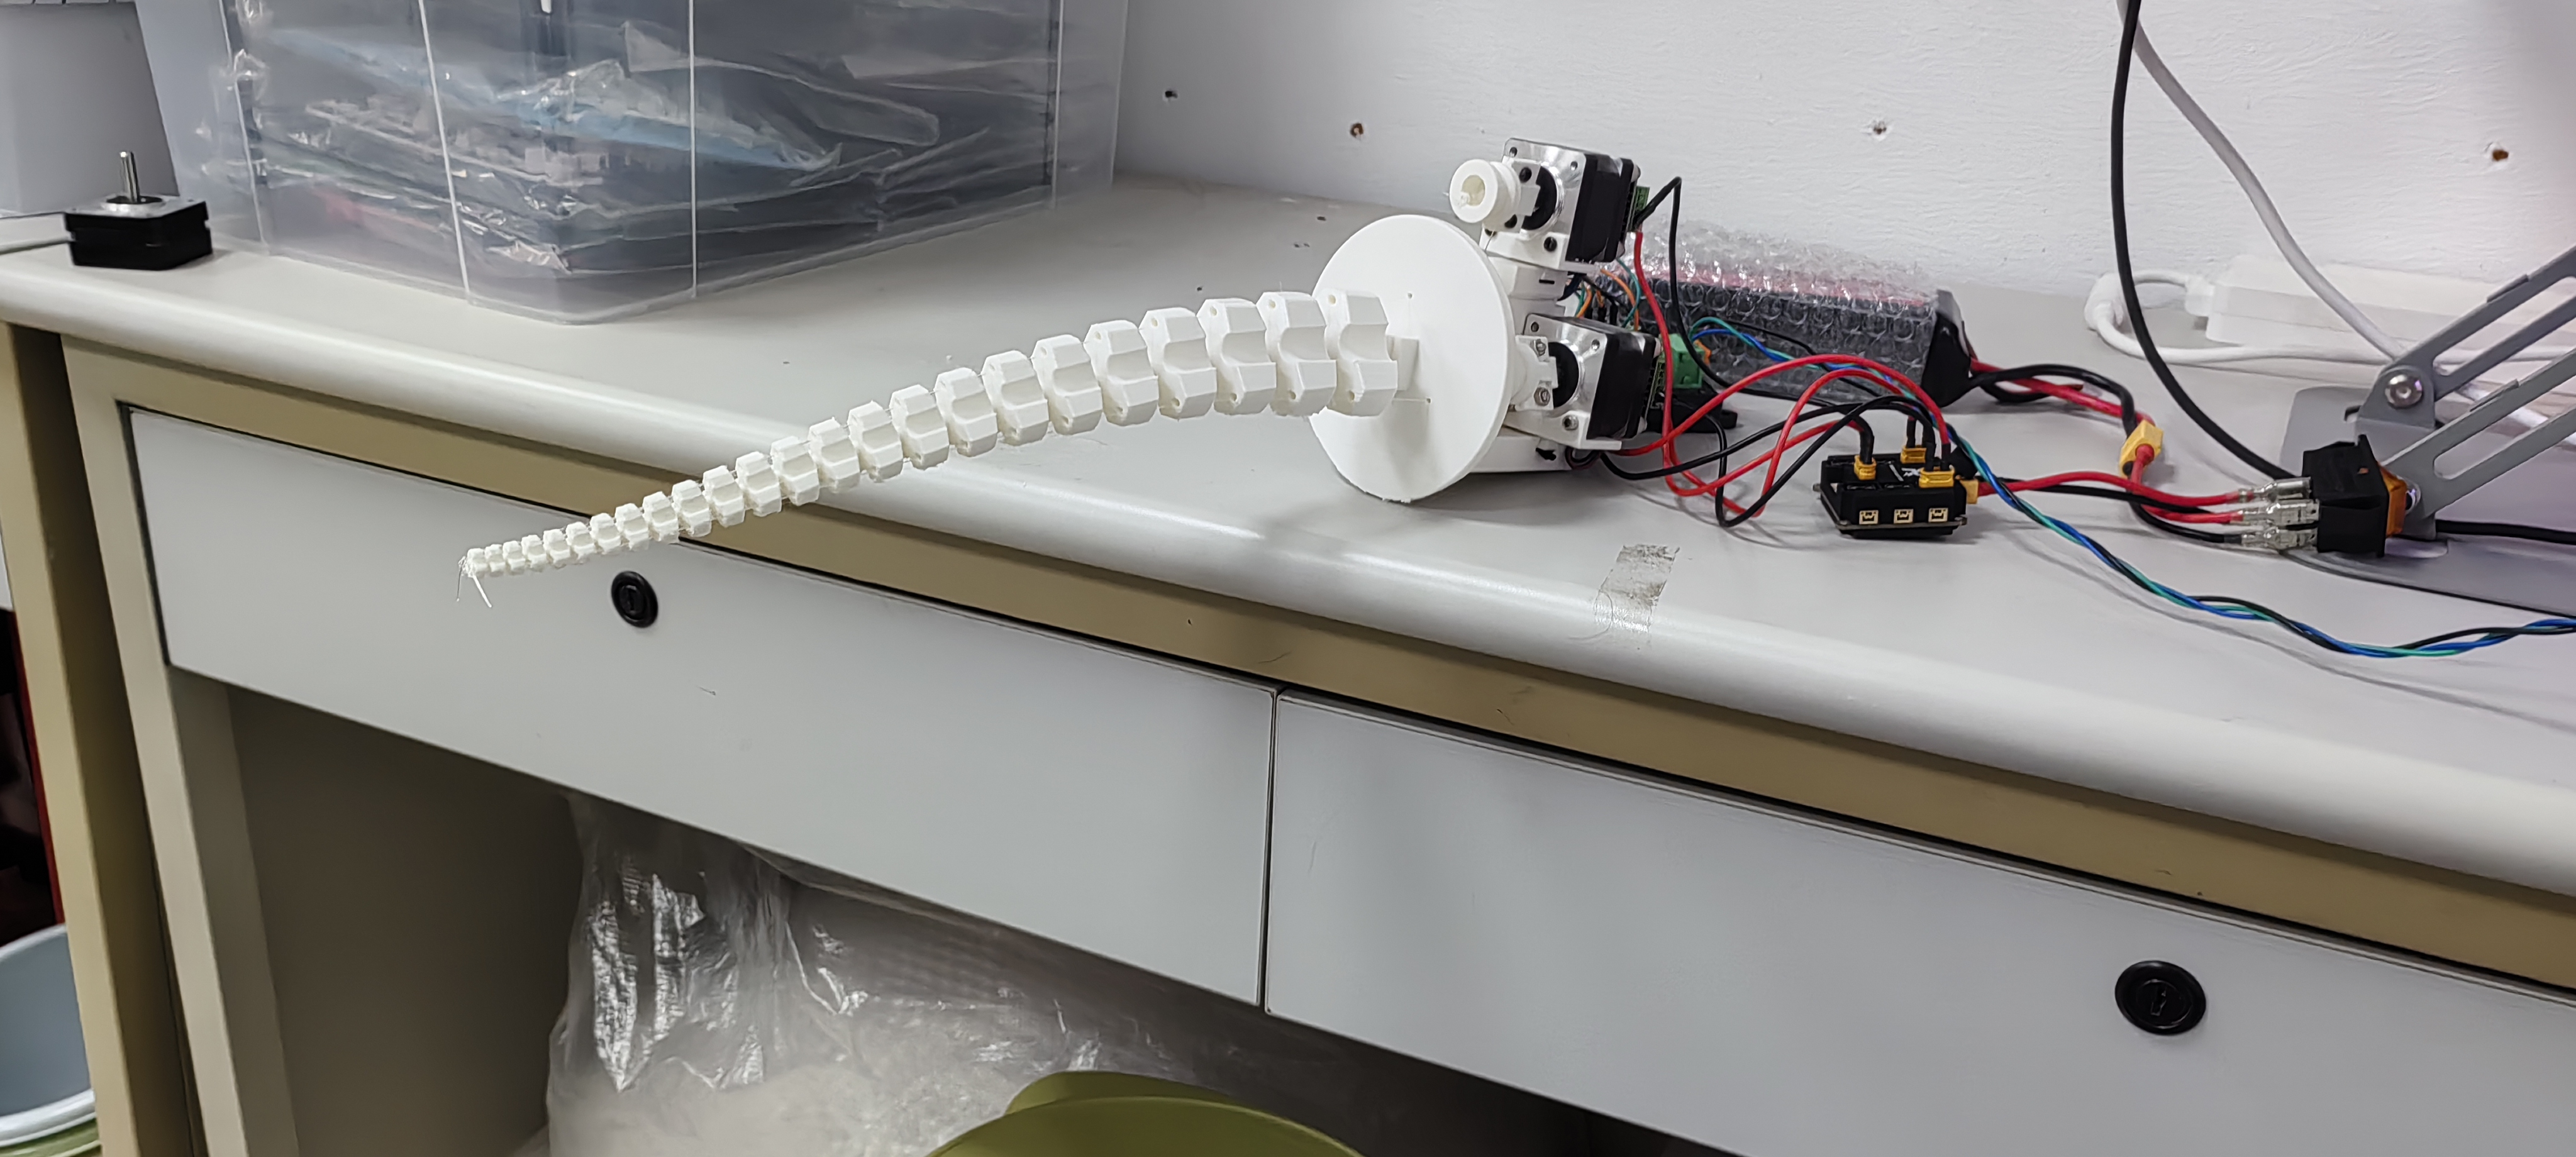
\includegraphics[width=0.6\linewidth]{微信图片_20260614013147_290_31.jpg}
\caption{SpiRobs 三绳驱动连续体机械臂样机总览}
\end{figure}

% ===================== 正文 =====================
\section{实验目的与任务}
\begin{itemize}[leftmargin=2em]
  \item 理解连续体机械臂区别于刚性串联臂的柔顺、分布式弯曲与冗余自由度特点，理解 SpiRobs 基于对数螺旋的仿生卷曲设计思想。
  \item 掌握柔性骨架、穿线盘、底座、绞盘等零件的三维建模与 TPU 柔性材料 3D 打印、装配与穿线预紧方法。
  \item 建立电机转角—绞盘半径—绳长变化—弯曲方向/角度的运动学近似关系，并完成电机连接、电路搭建与基础控制程序。
  \item 实现二维差动与三维全向弯曲控制，开展弯曲运动测试与柔性抓取拓展实验，分析误差来源并提出改进。
\end{itemize}

\section{实验原理}

\subsection{对数螺旋仿生设计}
SpiRobs 的核心思想是：当驱动绳收缩时，机械臂趋向预设的卷曲极限形态。将目标卷曲轨迹近似为对数螺旋
\begin{equation}
  r(\theta)=a\,e^{b\theta},
\end{equation}
其中 $a$ 决定初始半径、$b$ 决定卷曲的紧密程度。将螺旋按角度步长 $\Delta\theta$ 离散为一系列梯形"单元"，
并以中心螺旋边为轴镜像，展开为近直线的柔性主体。相邻单元的尺度比 $\gamma=e^{b\Delta\theta}$，
据此可得到锥角、末端/根部尺寸、单元数等派生量。改变主体宽度、厚度、缺口形状与穿线孔位置即可调节弯曲方向、
卷曲半径、末端力与可抓取范围。二维样机采用两根对置驱动绳，三维样机采用三根绳按 $120^\circ$ 分布。

本实验使用项目自带的 GUI 设计工具（\code{design-tool/}）完成上述参数化建模：左侧为二维极坐标/展开草图、
中部为 VTK 三维预览、右侧为参数面板，最终经 CadQuery 导出 STEP/STL（图~\ref{fig:design}）。

\begin{figure}[htbp]
\centering
\includegraphics[width=0.78\linewidth]{main-ui.png}
\par\medskip
\includegraphics[width=0.38\linewidth]{2d-sketch.png}\hspace{0.02\linewidth}\includegraphics[width=0.38\linewidth]{3d-model.png}
\caption{参数化设计工具：主界面（上）、二维展开草图（左下）与三维模型（右下）}
\label{fig:design}
\end{figure}

\subsection{绳驱动与绞盘换算}
绳驱动连续体臂通过驱动绳张力产生弯曲力矩。电机带动绞盘转动时，第 $i$ 根绳的长度变化可近似为
\begin{equation}
  \Delta l_i = r_s\,\theta_{m,i},
\end{equation}
其中 $r_s$ 为绞盘半径、$\theta_{m,i}$ 为电机转角。因此控制电机转角即可控制各绳的收/放量。
本实现用电机的\textbf{多圈编码器坐标}直接表示绳的"拉入量"，一圈对应 $N=16384$ 个编码器计数（与细分无关），
正值表示收紧（拉短）、负值表示放松（放长）。

\subsection{三绳恒曲率联动映射}
把整条触手看作一个\textbf{三自由度}对象：弯曲方向与大小（2 个自由度）合成弯曲向量 $(b_x,b_y)$，
加上整体收缩 $c$（1 个自由度），恰与三根驱动绳一一对应。设第 $i$ 根绳安装在横截面方位角 $\beta_i$
（三根互成 $120^\circ$），则恒曲率腱驱动模型给出各绳拉入量
\begin{equation}
  \ell_i \;=\; b_x\cos\beta_i + b_y\sin\beta_i + c \;=\; m\cos(\beta_i-\varphi) + c,
  \label{eq:fwd}
\end{equation}
其中弯曲量 $m=\sqrt{b_x^2+b_y^2}$、弯曲方向 $\varphi=\operatorname{atan2}(b_y,b_x)$。
弯曲项在 $120^\circ$ 均布下三绳之和为零（\emph{纯弯曲、不改变总长}），$c$ 为公共项（\emph{整体收缩}）。
即"朝某根绳的方向弯 = 收紧该绳、放松另两根"。该映射可逆，用于进入联动控制时由当前绳长反推弯曲状态：
\begin{equation}
  c=\frac{1}{3}\sum_i \ell_i,\qquad
  b_x=\frac{2}{3}\sum_i \ell_i\cos\beta_i,\qquad
  b_y=\frac{2}{3}\sum_i \ell_i\sin\beta_i.
\end{equation}

\subsection{非线性收放线整形}
式~\eqref{eq:fwd} 是线性对称的：收线与放线幅度相等。真机调试中发现这会使\textbf{放线侧过快松弛}，
驱动绳失张、姿态不受控。物理上柔性主体的中性轴并不位于几何中心、且小弯曲时外侧并不需要明显伸长，
因此应使放线在小弯曲时尽量少、大弯曲时才放足。为此只对\textbf{放线（负向）分量}施加随弯曲量增长的衰减增益，
而\textbf{收线侧保持线性}：
\begin{equation}
  \alpha(m)=\Big(\min(1,\;m/p_{\max})\Big)^{\,e-1},\qquad
  \ell_i' = \begin{cases}\ell_i, & \ell_i\ge 0\ (\text{收线})\\[2pt]\ell_i\cdot\alpha(m), & \ell_i<0\ (\text{放线})\end{cases}
  \label{eq:payout}
\end{equation}
其中 $p_{\max}$ 为单绳软上限，$e$ 为放线指数（\code{payout\_exp}，默认 $2$，$e=1$ 退回线性对称）。
此时放线量正比于 $m^{e}$（超线性），小弯曲几乎不放线、$m$ 到上限时回到线性满值。
表~\ref{tab:payout} 给出 $e=2$、朝绳 2 弯曲时的收/放比变化。

\begin{table}[htbp]
\centering
\caption{非线性收放线效果（朝绳 2 弯曲：绳 2 收线、绳 1/3 放线，$e=2$，$p_{\max}=1$）}
\label{tab:payout}
\footnotesize
\begin{tabular}{lccc}
\toprule
弯曲量 $m$（圈） & 0.2 & 0.6 & 1.0 \\
\midrule
收线（绳 2，圈）     & $+0.20$ & $+0.60$ & $+1.00$ \\
放线（绳 1/3，圈）   & $-0.02$ & $-0.18$ & $-0.50$ \\
收\,:\,放比          & $10\!:\!1$ & $3.3\!:\!1$ & $2\!:\!1$ \\
\bottomrule
\end{tabular}
\end{table}

最后做\textbf{协调截断}：若任一根 $|\ell_i'|>p_{\max}$，则三根等比缩小（而非单独削顶），以保持弯曲方向不变。
得到的目标再换算为电机坐标指令 $\mathrm{coord}_i = \mathrm{round}(d_i\cdot \ell_i'\cdot N)$（$N=16384$，
$d_i\in\{+1,-1\}$ 用于翻转线盘绕向，使"正拉入量"始终对应该绳收紧）。
上述联动映射、非线性放线整形与协调截断的实现见代码~\ref{lst:bend}（对应式~\eqref{eq:fwd} 与式~\eqref{eq:payout}）。

\begin{lstlisting}[language=Python,caption={三绳联动映射 + 非线性放线整形（SpiRob.pulls\_from\_bend）},label=lst:bend]
def pulls_from_bend(self, bx, by, contraction=0.0):
    m = math.hypot(bx, by)                                 # 弯曲量 m
    alpha = min(1.0, m / self.max_pull)**(self.payout_exp - 1)  # 放线衰减增益 alpha(m)
    pulls = []
    for a in self._cable_angles_rad:                       # 各绳安装角 beta_i
        bp = bx*math.cos(a) + by*math.sin(a)               # 线性弯曲分量
        if bp < 0:                                         # 仅放线(负向)侧
            bp *= alpha                                    # 非线性衰减
        pulls.append(bp + contraction)                     # 叠加整体收缩 c
    peak = max(abs(p) for p in pulls)
    if peak > self.max_pull:                               # 协调截断
        pulls = [p * self.max_pull / peak for p in pulls]  # 等比缩小, 保持弯曲方向
    return pulls
\end{lstlisting}

\section{实验设备与材料}
\begin{table}[htbp]
\centering
\caption{主要设备、元器件与软件}
\footnotesize
\begin{tabular}{p{3.6cm} p{11cm}}
\toprule
类别 & 内容 \\
\midrule
柔性主体（触手） & 拓竹 TPU for AMS 3D 打印的对数螺旋柔性骨架（一体连续弯曲） \\
刚性件（底座等） & 拓竹 PLA Basic 打印的底座、穿线端盘、绞盘、电机固定支座（见 \code{3D建模/}） \\
驱动 & 3 $\times$ MKS SERVO35D 闭环步进电机（板载 16384 线磁编码器，FOC 闭环；工作电流设为 1000\,mA） \\
通信 & USB 转 RS485 适配器（自动收发方向），三台并接同一总线，地址 1/2/3 \\
供电 & 12--24\,V 锂电池经分电板（RM 电调中心板）分 3 路给电机独立供电 \\
上位机 & PC + Python 3（\code{pyserial}），项目软件 \code{real\_deploy/} \\
其它 & 驱动绳、固定夹具、坐标纸/标定板、被抓取物体 \\
\bottomrule
\end{tabular}
\end{table}

\begin{figure}[htbp]
\centering
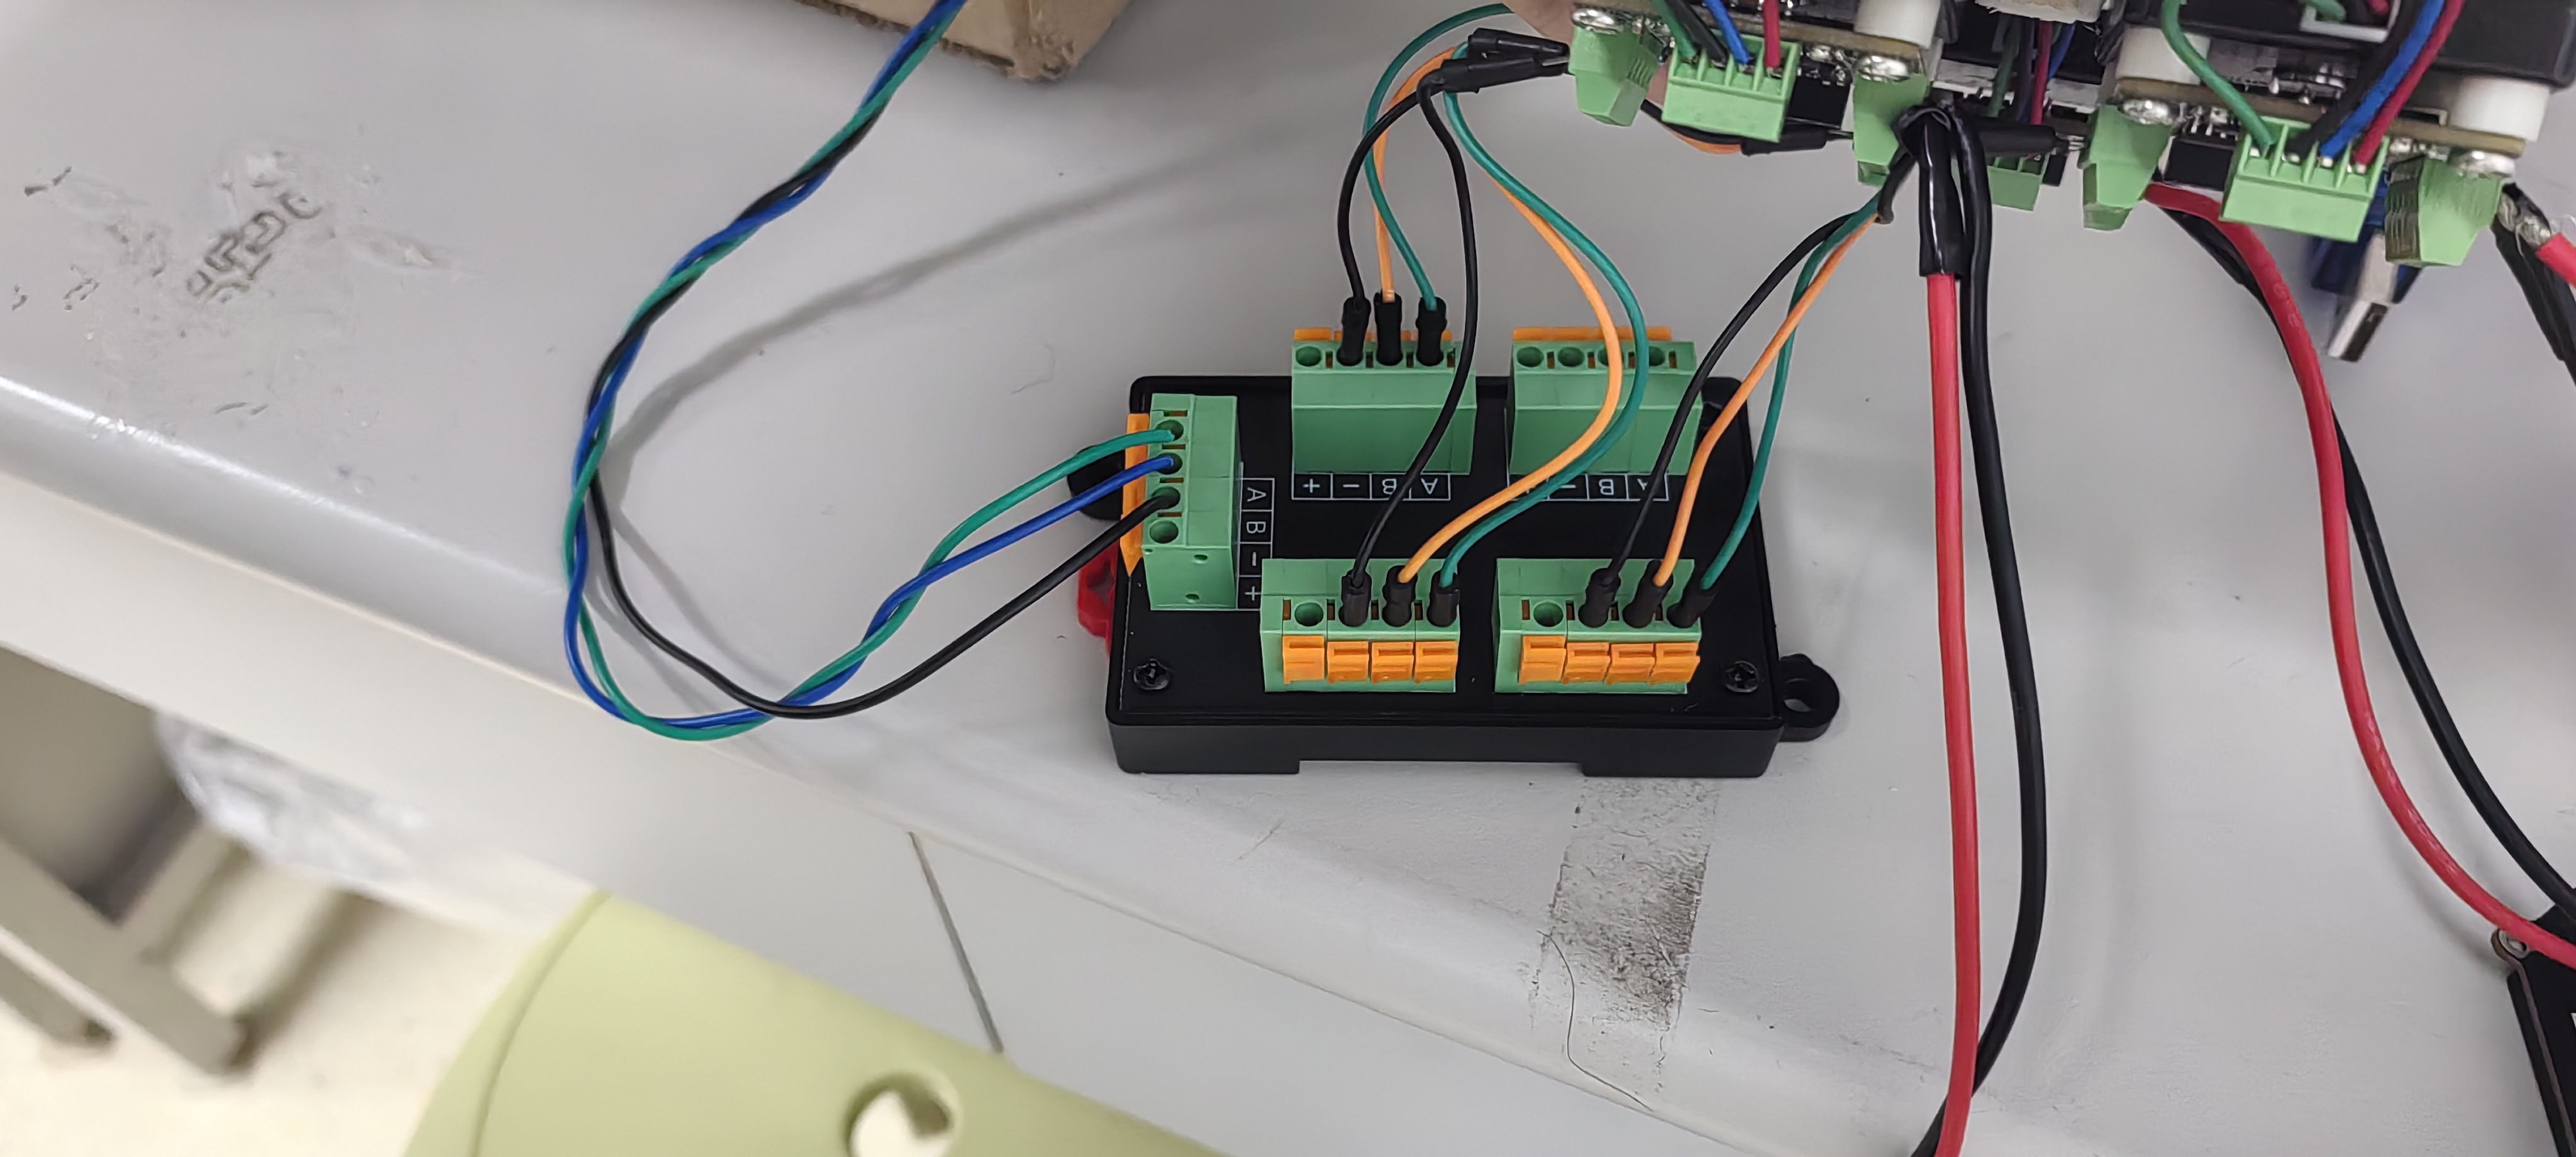
\includegraphics[width=\linewidth]{微信图片_20260614022130_296_31.jpg}\par\medskip
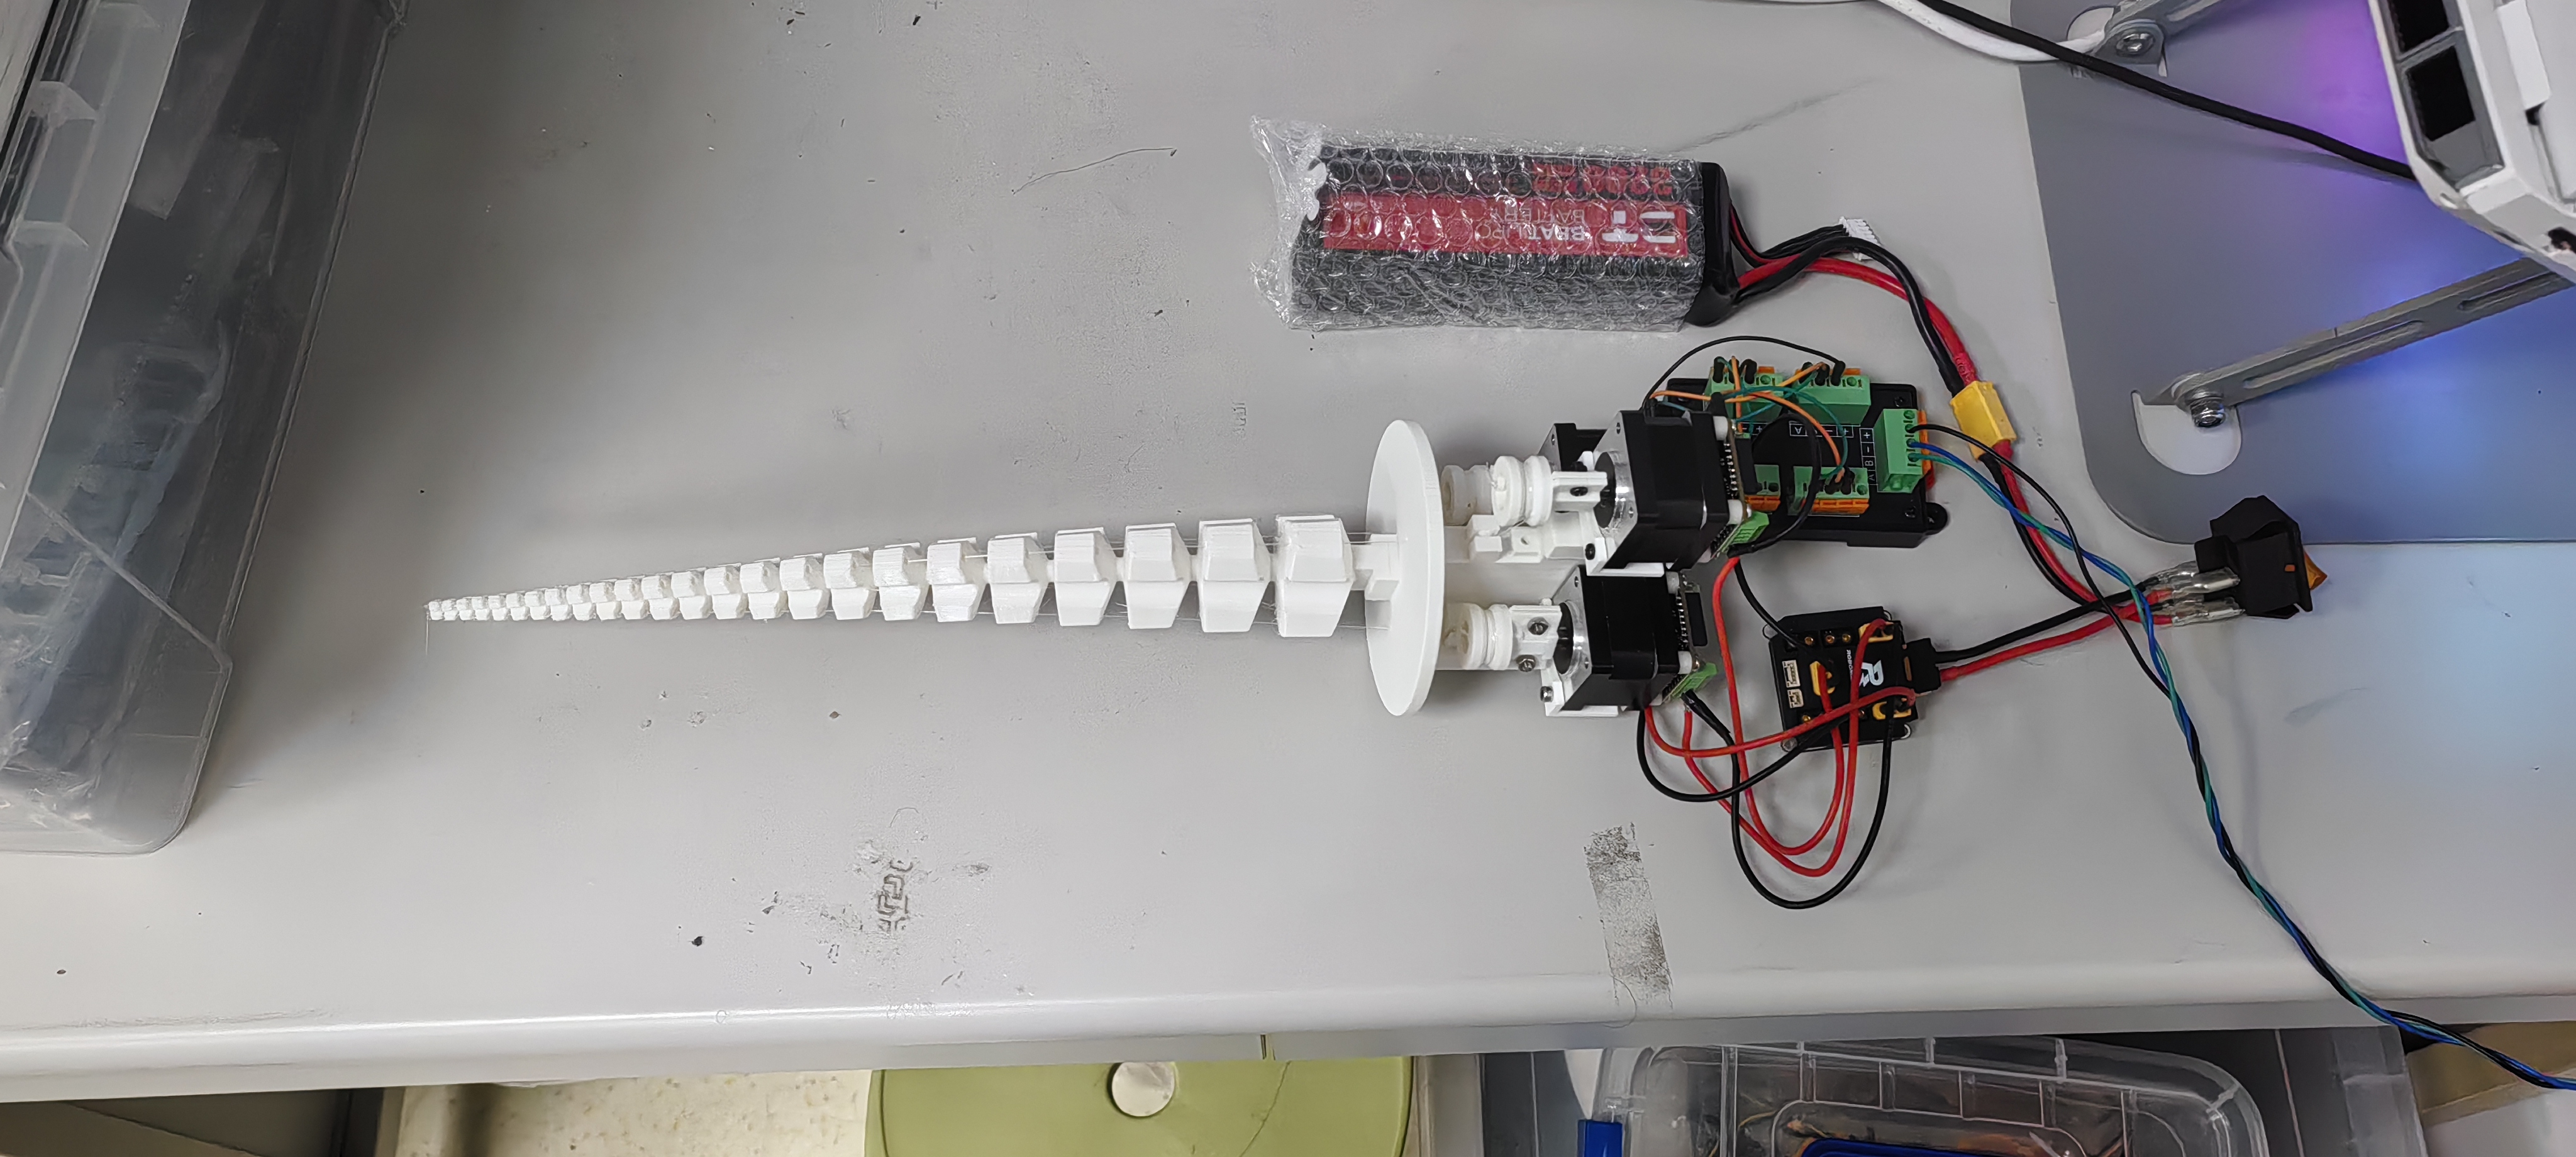
\includegraphics[width=\linewidth]{微信图片_20260614013141_287_31.jpg}\par\medskip
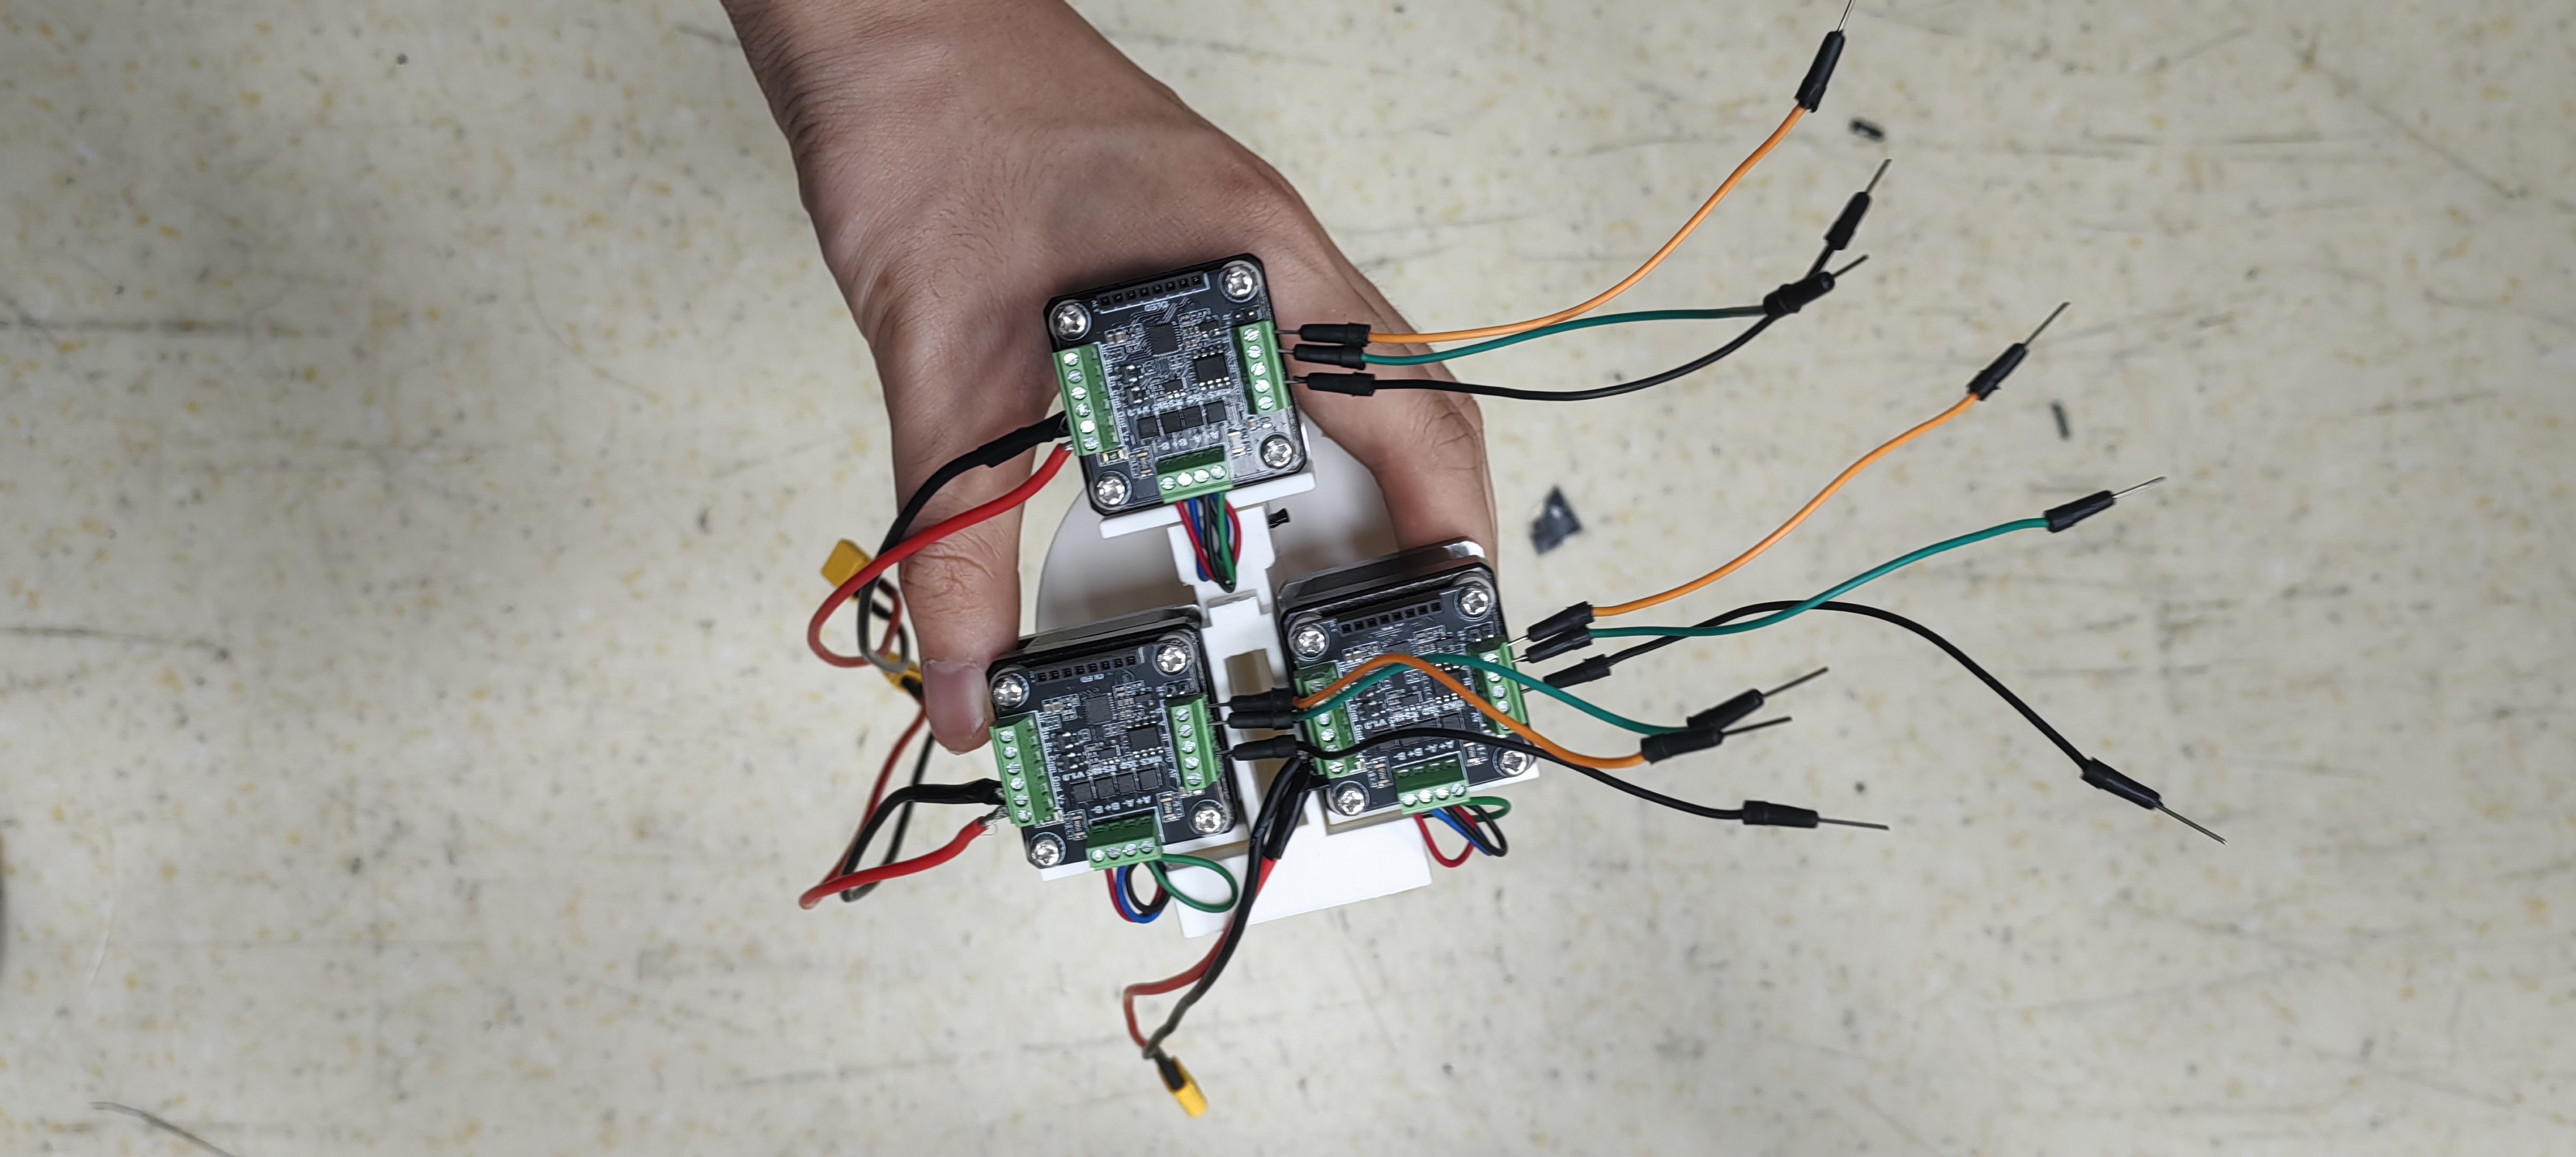
\includegraphics[width=\linewidth]{微信图片_20260614022132_297_31.jpg}
\caption{硬件搭建：三电机 RS485 同总线（上）、锂电池经分电板三路供电（中）、电机驱动板接线（下）}
\label{fig:hw}
\end{figure}

\section{实验内容与步骤}

\subsection{结构设计与三维建模}
在设计工具中设定样机类型（三维全向弯曲）、总长、截面直径与驱动绳数量（3 根），
设置弹性体厚度与对数螺旋参数 $a,b,\Delta\theta$，布置三个相隔 $120^\circ$ 的穿线孔并在端部设置绳端固定点；
设计绞盘半径以便电机转角换算为绳长变化，保证电机轴线、绞盘与导向孔对齐；导出 STL 并检查穿线孔贯通与可拆装性。

具体地，本样机在 GUI 中将弹性层参数 \code{elastic} 设为 $20$（即 $20\%$），并联调螺旋参数 $a$、$b$，
使界面派生显示的\textbf{触手长度}（Robot Length）落在 $20\sim25\,$cm、\textbf{最底部一节截面直径}（Base Size）
落在 $40\sim50\,$mm 区间，从而兼顾足够的卷曲行程与根部刚度/绞盘力臂。

\subsection{3D 打印与装配}
触手柔性主体用\textbf{拓竹 TPU for AMS} 打印（适当层高、壁厚与填充以兼顾弯曲刚度与回弹），
底座、绞盘与支架用\textbf{拓竹 PLA Basic} 打印；去除支撑与毛刺、检查穿线孔通畅；
将柔性主体固定于底座、保证中性轴竖直、端面平整以避免初始偏弯；驱动绳由末端固定点穿过各级导向孔至底座绞盘；
轻拉各绳做\textbf{初始预紧}使主体保持竖直后再固定绳端。

\subsection{绳驱动系统连接与预紧}
将三根绳分别绕至三台电机绞盘并固定；按图~\ref{fig:hw} 完成 RS485 同总线并联（A--A、B--B、末端 $120\,\Omega$ 跳线）
与分电板三路供电；确认共地、电压与极性后上电。三台电机出厂地址设为 1/2/3。

\subsection{控制系统实现}
控制软件 \code{real\_deploy/} 分三层：
\begin{itemize}[leftmargin=2em]
  \item \textbf{\code{MksBus}}：管理一条 RS485 总线，封装 MKS 自定义协议帧
        （下行 \code{FA addr code data...\ checksum}、上行 \code{FB ...}，大端，校验和 $=\sum(\text{字节})\,\&\,\text{0xFF}$），半双工一问一答。
  \item \textbf{\code{MksServo}}：单台电机指令——设工作模式 \code{82H}（总线 FOC \code{SR\_vFOC}）、使能 \code{F3H}、
        置零 \code{92H}、坐标绝对运动 \code{F5H}（支持运动中实时更新）、读坐标 \code{31H}、读转速/堵转/IO、
        编码器校准 \code{80H}、设工作电流 \code{83H}。
  \item \textbf{\code{SpiRob}}：三绳协调层，实现式~\eqref{eq:fwd}--\eqref{eq:payout} 的联动映射、协调截断、置零/回零、诊断与电流设置。
\end{itemize}
其中 \code{MksBus} 的帧组装与校验实现如代码~\ref{lst:frame}（下行帧 \code{FA+地址+命令+数据+校验和}，
校验和为各字节之和按位与 \code{0xFF}，半双工读取应答后校验帧头/地址/命令/校验和）。

\begin{lstlisting}[language=Python,caption={RS485 帧组装与校验和（MksBus.transfer 摘录）},label=lst:frame]
def transfer(self, addr, code, data=b"", resp_data_len=1):
    body  = bytes([0xFA, addr, code]) + bytes(data)   # 帧头FA + 地址 + 命令 + 数据
    frame = body + bytes([sum(body) & 0xFF])          # 校验和 = 各字节之和 & 0xFF
    self.ser.reset_input_buffer()
    self.ser.write(frame)
    resp = self.ser.read(3 + resp_data_len + 1)       # 应答: FB 地址 命令 数据... 校验
    # 校验 帧头(0xFB)/地址/命令/校验和 后, 返回数据段:
    return resp[3:-1]
\end{lstlisting}

控制链路（联动模式）为：按键 $\to$ 弯曲状态 $(b_x,b_y,c)$ $\to$ 恒曲率映射 $\to$ 非线性放线整形
$\to$ 协调截断 $\to$ 三绳目标 $\to$ \code{F5} 坐标绝对运动 $\to$ 电机。
上位机用终端 cbreak 模式做\textbf{单键即时}采集（无需回车、保留 \code{Ctrl+C} 急停），
并把键盘连发合并为一次目标更新（松手即停、无拖尾）。提供两种模式：
\begin{itemize}[leftmargin=2em]
  \item \textbf{触手联动（推荐）}：\code{WASD} 控制弯曲方向与大小、\code{i/k} 控制整体收缩、\code{[}/\code{]} 实时调节放线指数；
  \item \textbf{单绳直控}：\code{u/i/o} 收、\code{j/k/l} 放，逐绳增量，用于调试与找零位。
\end{itemize}

触手联动键盘遥操作的主循环如代码~\ref{lst:loop}：终端设为 cbreak（单键即时、保留 \code{Ctrl+C}），
合并连发按键更新弯曲状态 $(b_x,b_y,c)$ 后调用 \code{set\_bend} 联动下发（内部按 \code{max\_pull} 截断，即限位策略）；
\code{Ctrl+C} 触发急停且留在循环。

\begin{lstlisting}[language=Python,caption={触手联动键盘遥操作主循环（tentacle\_control 摘录）},label=lst:loop]
def tentacle_control(robot):                    # 触手联动键盘主循环
    bx, by, c = robot.bend_from_pulls(robot.read_pull())  # 从当前姿态接续
    with _raw_terminal() as fd:                 # 终端设为 cbreak (保留信号)
        while True:
            try:
                dirty = False
                for ch in _iter_keys(_read_key_batch(fd)):  # 合并连发按键
                    if   ch == 'q': return                  # 退出
                    elif ch == 'w': by += step; dirty = True  # 弯曲方向/大小
                    elif ch == 's': by -= step; dirty = True
                    elif ch == 'a': bx -= step; dirty = True
                    elif ch == 'd': bx += step; dirty = True
                    elif ch == 'i': c  += step; dirty = True  # 整体收缩
                    elif ch == 'k': c  -= step; dirty = True
                    elif ch == 'z': robot.set_zero_here(); bx=by=c=0.0; dirty=True
                if dirty:
                    robot.set_bend(bx, by, c)   # 三绳联动下发(内部按 max_pull 截断)
            except KeyboardInterrupt:           # Ctrl+C: 急停, 留在循环
                robot.estop()
\end{lstlisting}

\subsection{标定与零位}
\begin{enumerate}[leftmargin=2em]
  \item \textbf{绕向 $d_i$}：逐根给小的正拉入量，观察该绳是否"收紧"；若相反则将该路 $d_i$ 置 $-1$（\code{--dirs}）。
  \item \textbf{安装角 $\beta_i$}：只拉某一根绳，触手即朝该绳方向倒；记下其物理方位角即为 $\beta_i$。
        本样机三绳位于 8/12/4 点方向，按 $\beta=(90^\circ-30^\circ\times\text{钟点})\bmod 360^\circ$ 换算得
        $\beta=(210^\circ,90^\circ,330^\circ)$（\code{--cable-angles}）。
  \item \textbf{编码器校准}：必要时空载执行 \code{80H}（对应上位机 Cal）重学磁编码器零位。
  \item \textbf{置零}：在中性/绷直姿态执行 \code{92H} 置零，之后所有绝对位置以此为基准。
\end{enumerate}

\section{实验结果与分析}

\subsection{全向弯曲与自由度验证}
完成标定后进入联动模式，\code{WASD} 可驱动触手向任意方向连续弯曲，\code{i/k} 实现整体收缩/伸展，
三绳由式~\eqref{eq:fwd} 协调收放、不再各自单独控制。例如朝 $+Y$（$12$ 点、绳 2 方向）弯曲时，
绳 2 收线、绳 1/3 协调放线，末端沿预期方向倾倒，验证了三绳到三自由度的映射正确性。

\subsection{非线性收放线的效果}
将放线指数从 $e=1$（线性对称）调至 $e=2$ 后，小弯曲阶段放线量大幅减小（表~\ref{tab:payout}：$m=0.2$ 时由
$-0.10$ 降到 $-0.02$，收/放比由 $2\!:\!1$ 提升到 $10\!:\!1$），有效避免了驱动绳过早失张；
随弯曲增大放线逐渐放足，$m$ 到上限时与线性一致。该整形显著改善了大角度卷曲时的姿态可控性与绳张力保持。

\subsection{柔性抓取拓展}
在弯曲控制基础上演示了\textbf{从上方}与\textbf{从下方}对物体的抓取（图~\ref{fig:grasp}）：利用对数螺旋形态的卷曲包络特性，
触手通过自身形变贴合并约束目标物，完成"接近—接触—卷曲—提升—释放"流程，体现了柔性连续体相比刚性夹爪
对不同尺寸/外形物体的适应能力。

\begin{figure}[htbp]
\centering
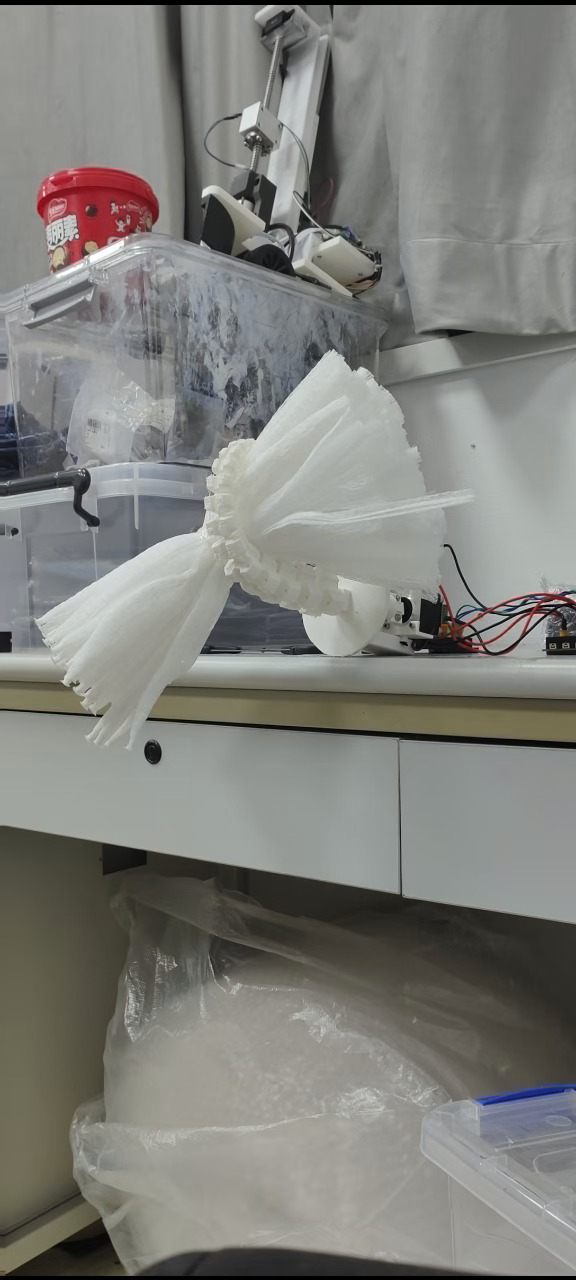
\includegraphics[height=11.5cm]{grasp_up.jpg}\hspace{0.04\linewidth}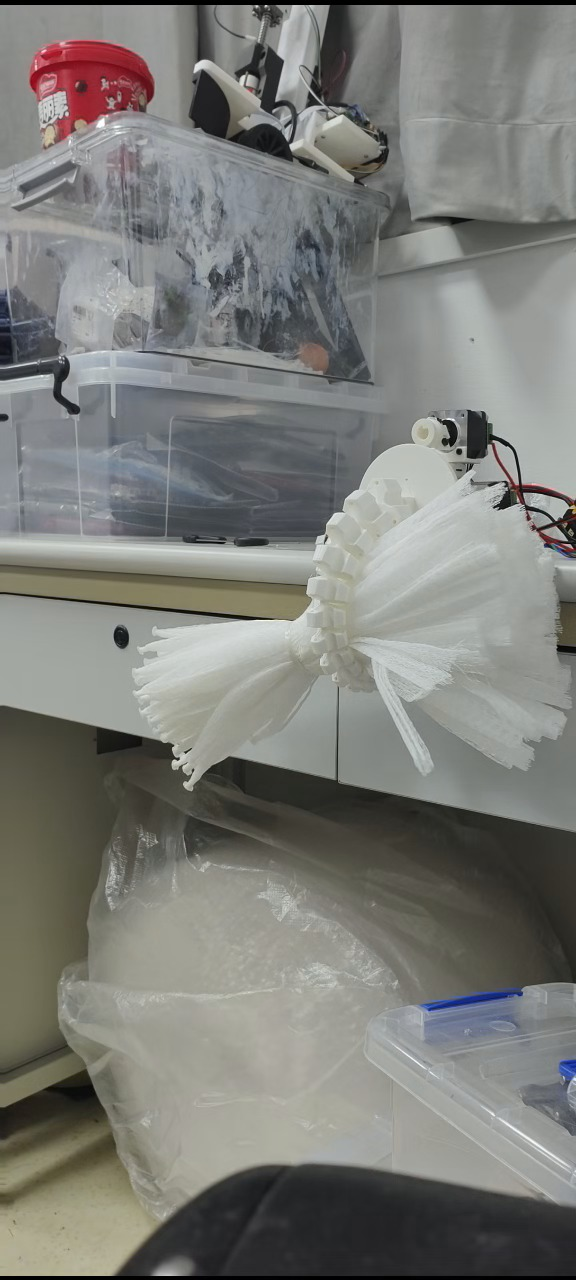
\includegraphics[height=11.5cm]{grasp_down.jpg}
\caption{柔性抓取演示：向上抓取（左）与向下抓取（右）}
\label{fig:grasp}
\end{figure}

\subsection{安全与诊断机制}
软件设单绳软上限 \code{max\_pull} 防止误操作拉断；任意时刻 \code{Ctrl+C} 触发急停（保留信号、不松轴），
退出统一执行"先停车再松轴"；\code{diag} 命令一次读出运行状态、坐标、堵转标志、限位输入与限位/保护配置，
便于区分"被保护停"与"到目标停"。调试中曾出现"正反转一定圈数即停"，经 \code{diag} 与分析确认主要为软件
\code{max\_pull} 截断而非电机侧限位。为增大力矩、保证绳张力，本样机已将工作电流由 35D 默认的 $800\,$mA
上调至 $1000\,$mA（\code{83H}，可经 \code{--current 1000} 在启动时设定）。

\section{误差来源与改进}
\begin{itemize}[leftmargin=2em]
  \item \textbf{绳驱动摩擦与松弛}：导向孔摩擦、绳弹性与初始预紧不均会导致弯曲滞后与方向偏差；改进：优化孔位与导向、统一预紧。
  \item \textbf{中性轴非中心}：实际中性轴偏离几何中心，使线性收放线不准——已用非线性放线整形缓解，可进一步按实测标定曲线。
  \item \textbf{开环控制}：当前为开环位置控制，无末端反馈，存在累积误差；改进：引入动捕/IMU/电流反馈实现闭环。
  \item \textbf{标定误差}：$\beta_i$、$d_i$、绞盘半径与零位的人工标定误差影响方向精度；改进：增加自动标定流程。
  \item \textbf{材料与结构}：TPU 刚度、疲劳与打印方向影响回弹与寿命；改进：调整材料硬度、穿线孔位置或采用多段串联结构。
  \item \textbf{电机扭矩不足与结构柔度欠佳（主要失效模式）}：电机扭矩偏小，叠加 \code{elastic} 参数调节欠佳，
        使触手各节连接处偏粗、整体柔软程度略低；在\textbf{深度弯曲}或\textbf{带载抓取}时所需牵引力显著增大，
        电机拉力不足、容易\textbf{堵转}而无法牵引到位。改进：进一步增大工作电流或更换更大扭矩的电机、增大绞盘力臂；
        重调 \code{elastic} 与螺旋参数 $a,b$ 以减小连接处截面、提升整体柔顺性，降低同等弯曲所需的绳张力。
\end{itemize}

\section{实验安全注意事项}
电机通电可能突然转动，调试前固定样机与电机座，勿将手指置于绞盘/绳/关节之间；连接控制板、驱动器与电源前确认
电压、电流、极性与共地，改线必先断电；预紧与大角度弯曲可能断绳回弹，应限制最大张力、勿正对绳索方向观察、
首次驱动低速小行程；多人协作时由专人负责上电与启动，其余人员保持安全距离。

\section{结论}
本实验完整实现了 SpiRobs 绳驱动连续体机械臂的设计—制作—驱动—标定—控制全流程。核心贡献在控制层：
将三电机抽象为触手的三自由度任务空间，建立了恒曲率腱驱动联动映射，并针对真机失张问题提出非线性收放线整形；
配合单键实时遥操作、标定与安全/诊断机制，样机实现了全向弯曲与柔性抓取。后续可在闭环反馈、自动标定与
多段/多机协作方向继续拓展。

\begin{thebibliography}{9}
\bibitem{spirobs} Wang, Zhanchi, Nikolaos M. Freris, and Xi Wei.
``SpiRobs: Logarithmic spiral-shaped robots for versatile grasping across scales.'' \emph{Device} 3.4 (2025).
\end{thebibliography}

\end{document}
